\begin{figure}[hbt]
\begin{minipage}{0.5\textwidth}
 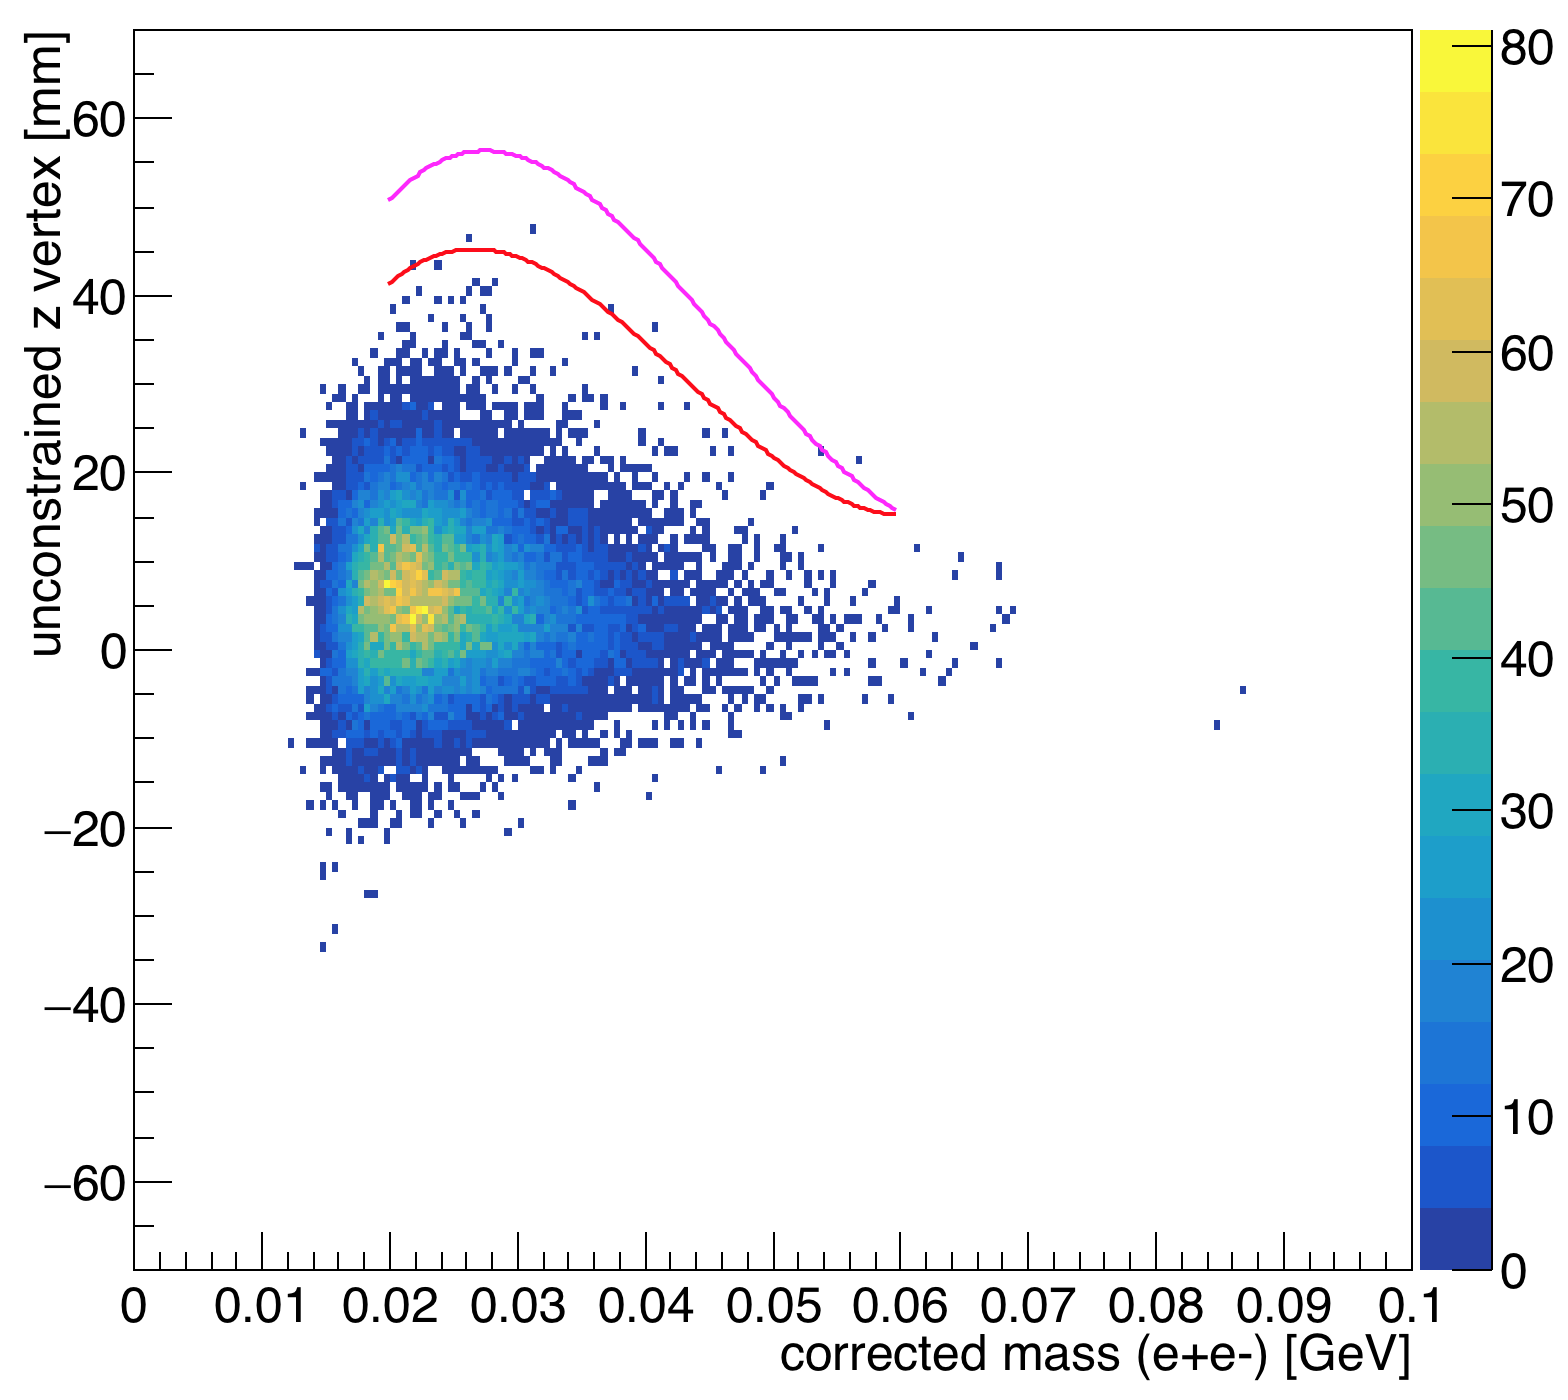
\includegraphics[width=\textwidth]{pics/appendix/zVm_L1L2_0p5_bl.png}
\end{minipage}\hfill\begin{minipage}{0.5\textwidth}
 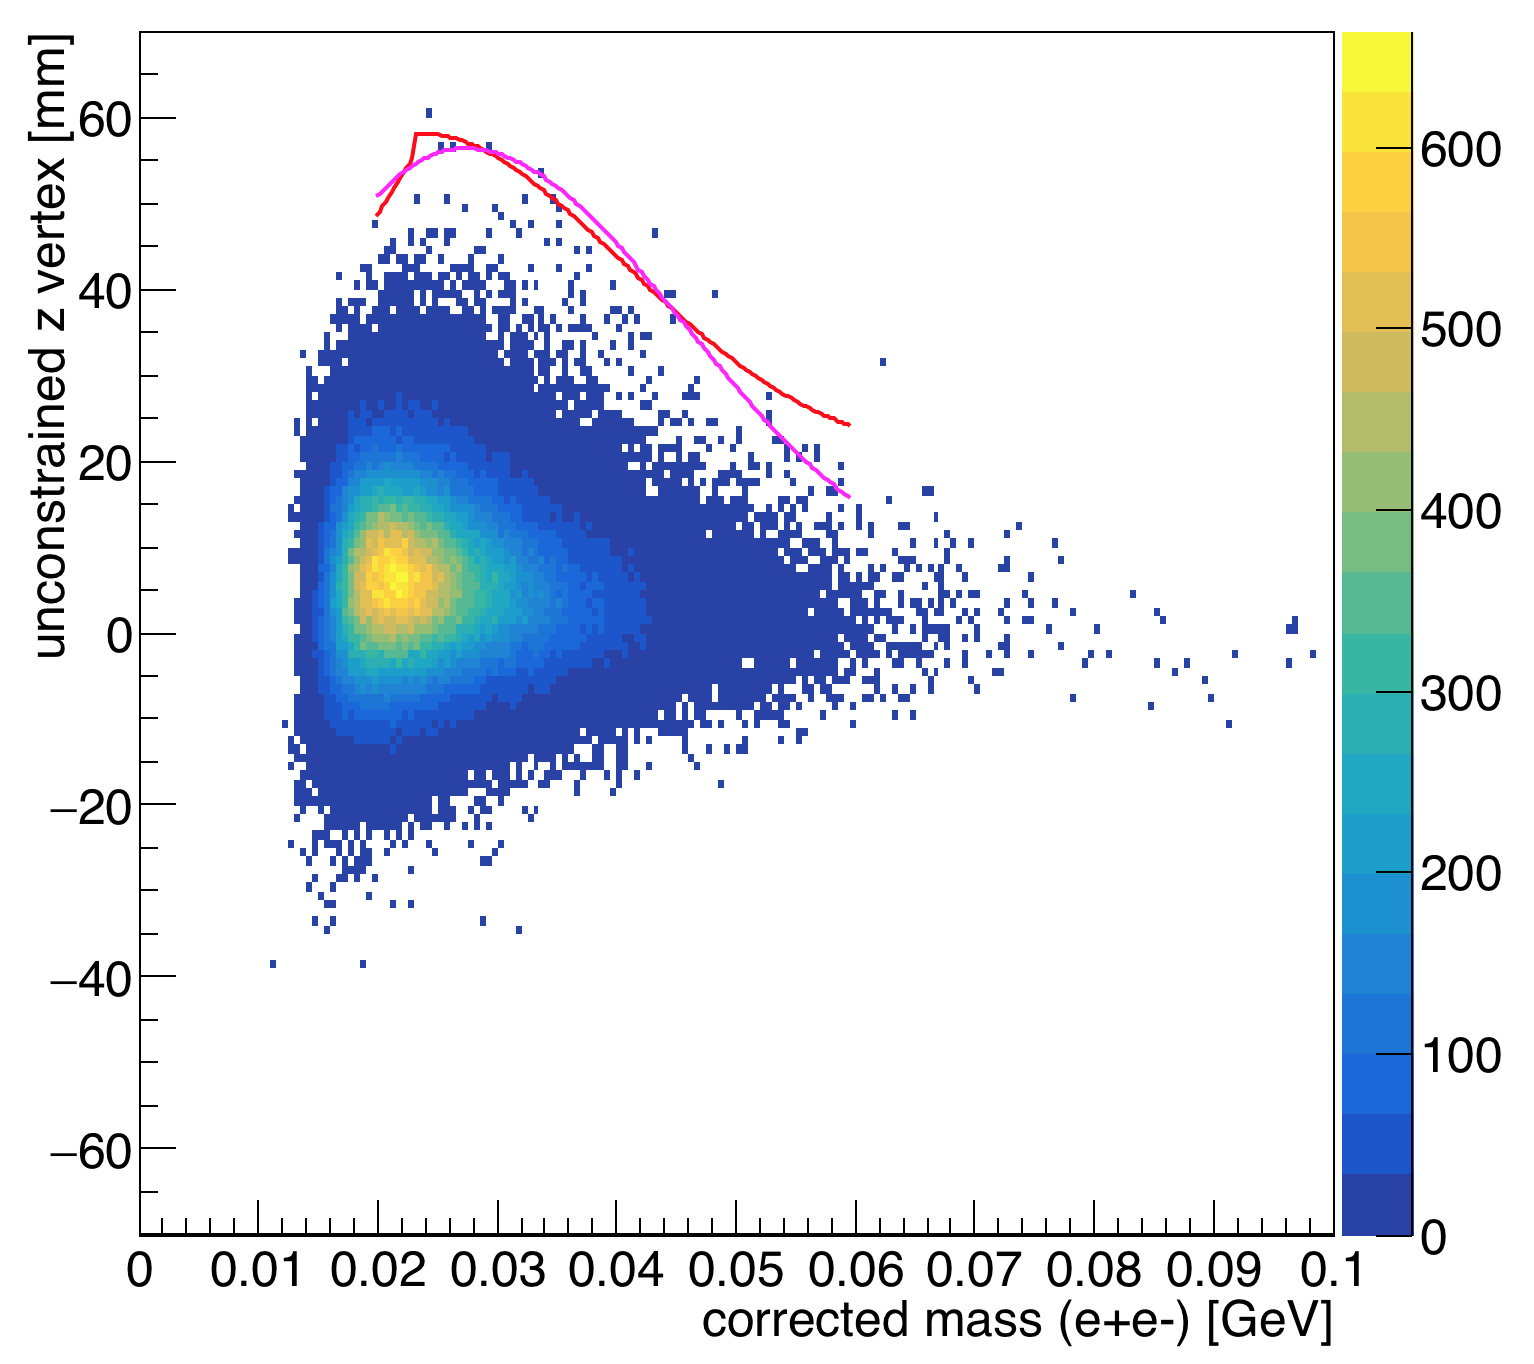
\includegraphics[width=\textwidth]{pics/appendix/zVm_L1L2_0p5_ub.png}
 \end{minipage}
  \caption[$z$ vertex and mass distribution for the L1L2 data set with the SVT at $\pm0.5$~mm]{The unconstrained $z$ vertex position for the L1L2 data set with the SVT at $\pm0.5$~mm is shown as a function of the corrected mass of the $e^+e^-$ pair where one track has a hit in Layer 1 and the other track does not pass through the active region of Layer 1. The $zCut$ as measured for this data is shown in red and corresponds to the full 100$\%$ data set where there is less than 0.5 background event beyond. The projected $zCut$ from the 10$\%$ of the data is shown in magenta. The relevant mass range used to measure $zCut$ is from 0.02--0.06~GeV based on measured statistics. The 10$\%$ sample for tuning cuts is shown on the left, and the full 100$\%$ of the data is shown on the right.}
  \label{fig:zvm_l1l2}
\end{figure}
\begin{figure}[htb]
  \centering
      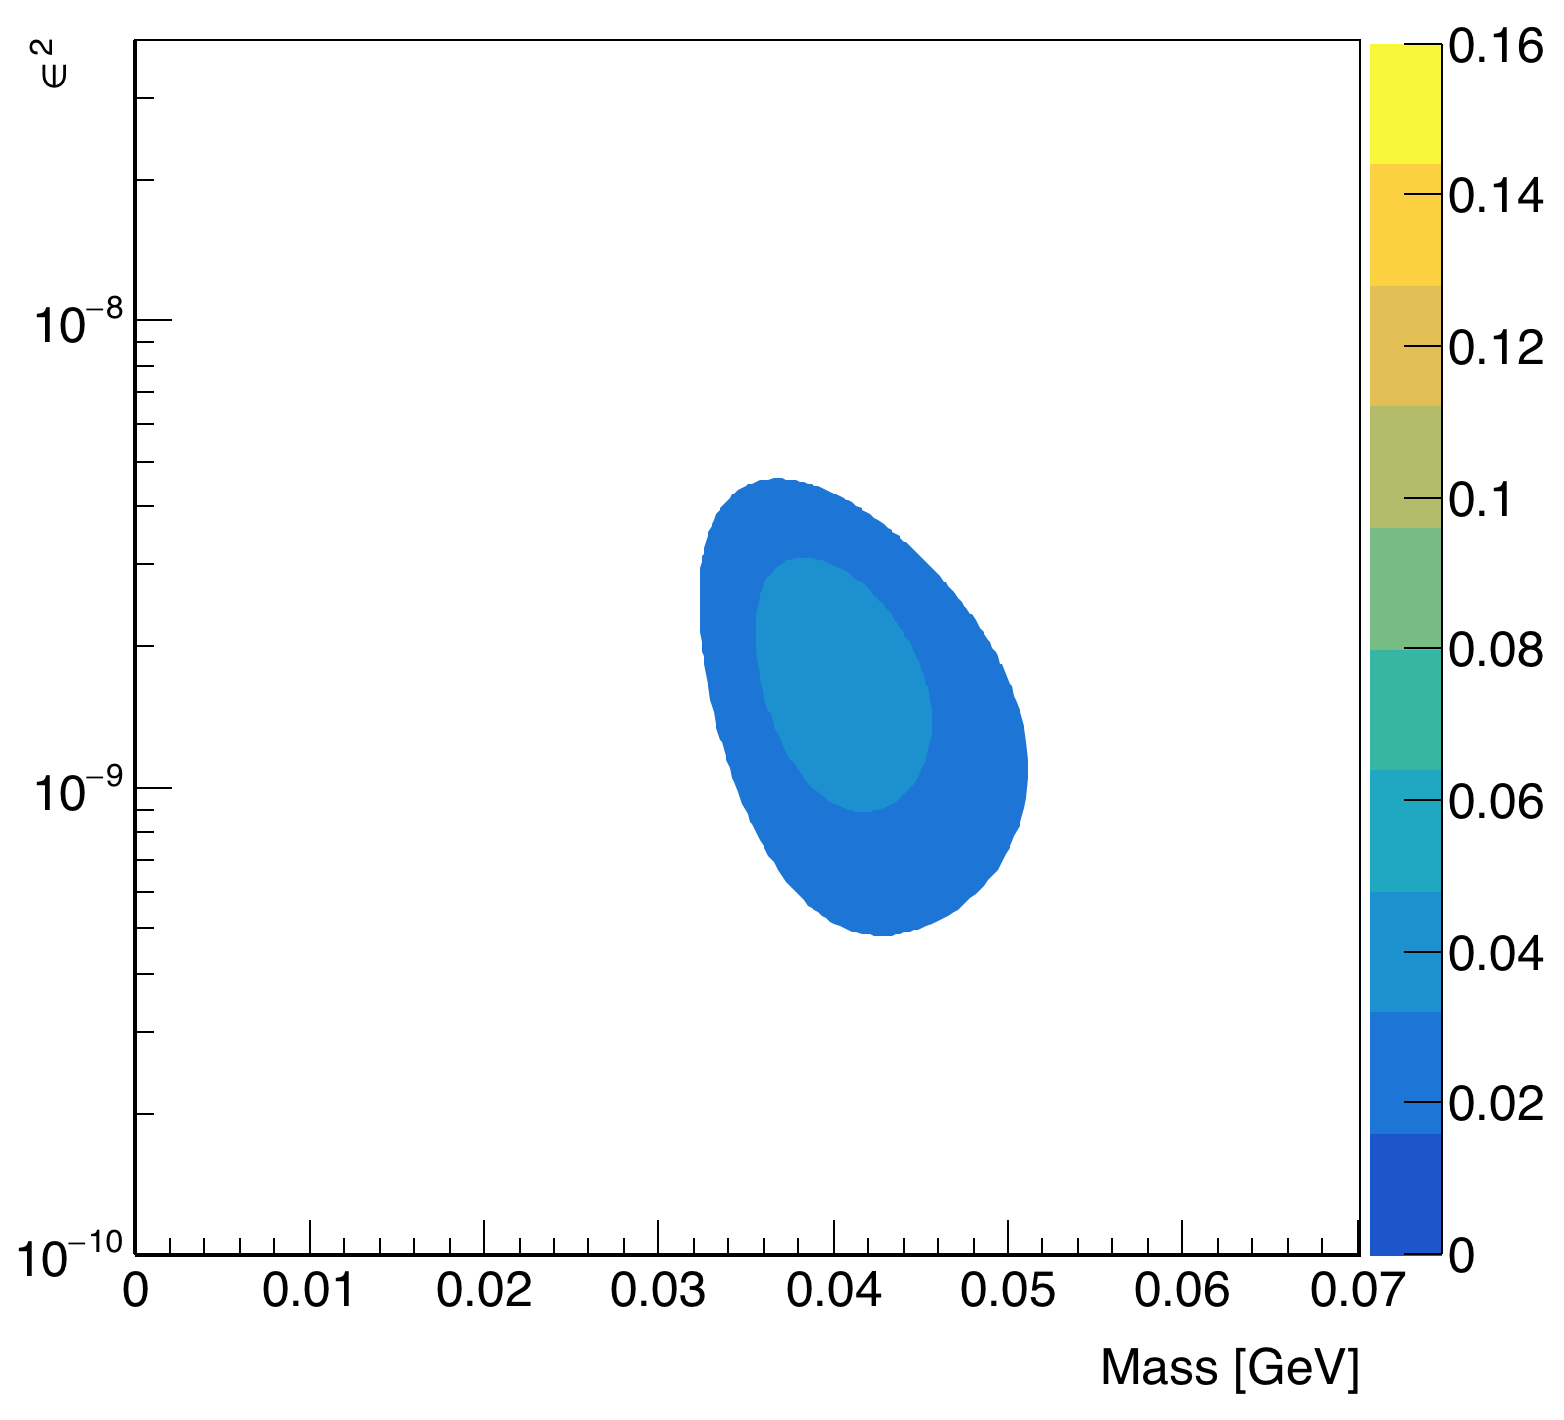
\includegraphics[width=0.5\textwidth]{pics/appendix/reachL1L2_0p5.png}
  \caption[Expected detectable $A^{\prime}$ signal yield from the L1L2 data at 0.5~mm.]{The expected number of detectable $A^{\prime}$ signal events from the L1L2 data set with the SVT at $\pm0.5$~mm is 0.04 events, and the distribution for coupling and mass space is shown. This calculation uses the $zCut$ shown in Figure~\ref{fig:zvm_l1l2}.}
  \label{fig:rl1l20p5}
\end{figure} 
\begin{figure}[hbt]
\begin{minipage}{0.5\textwidth}
 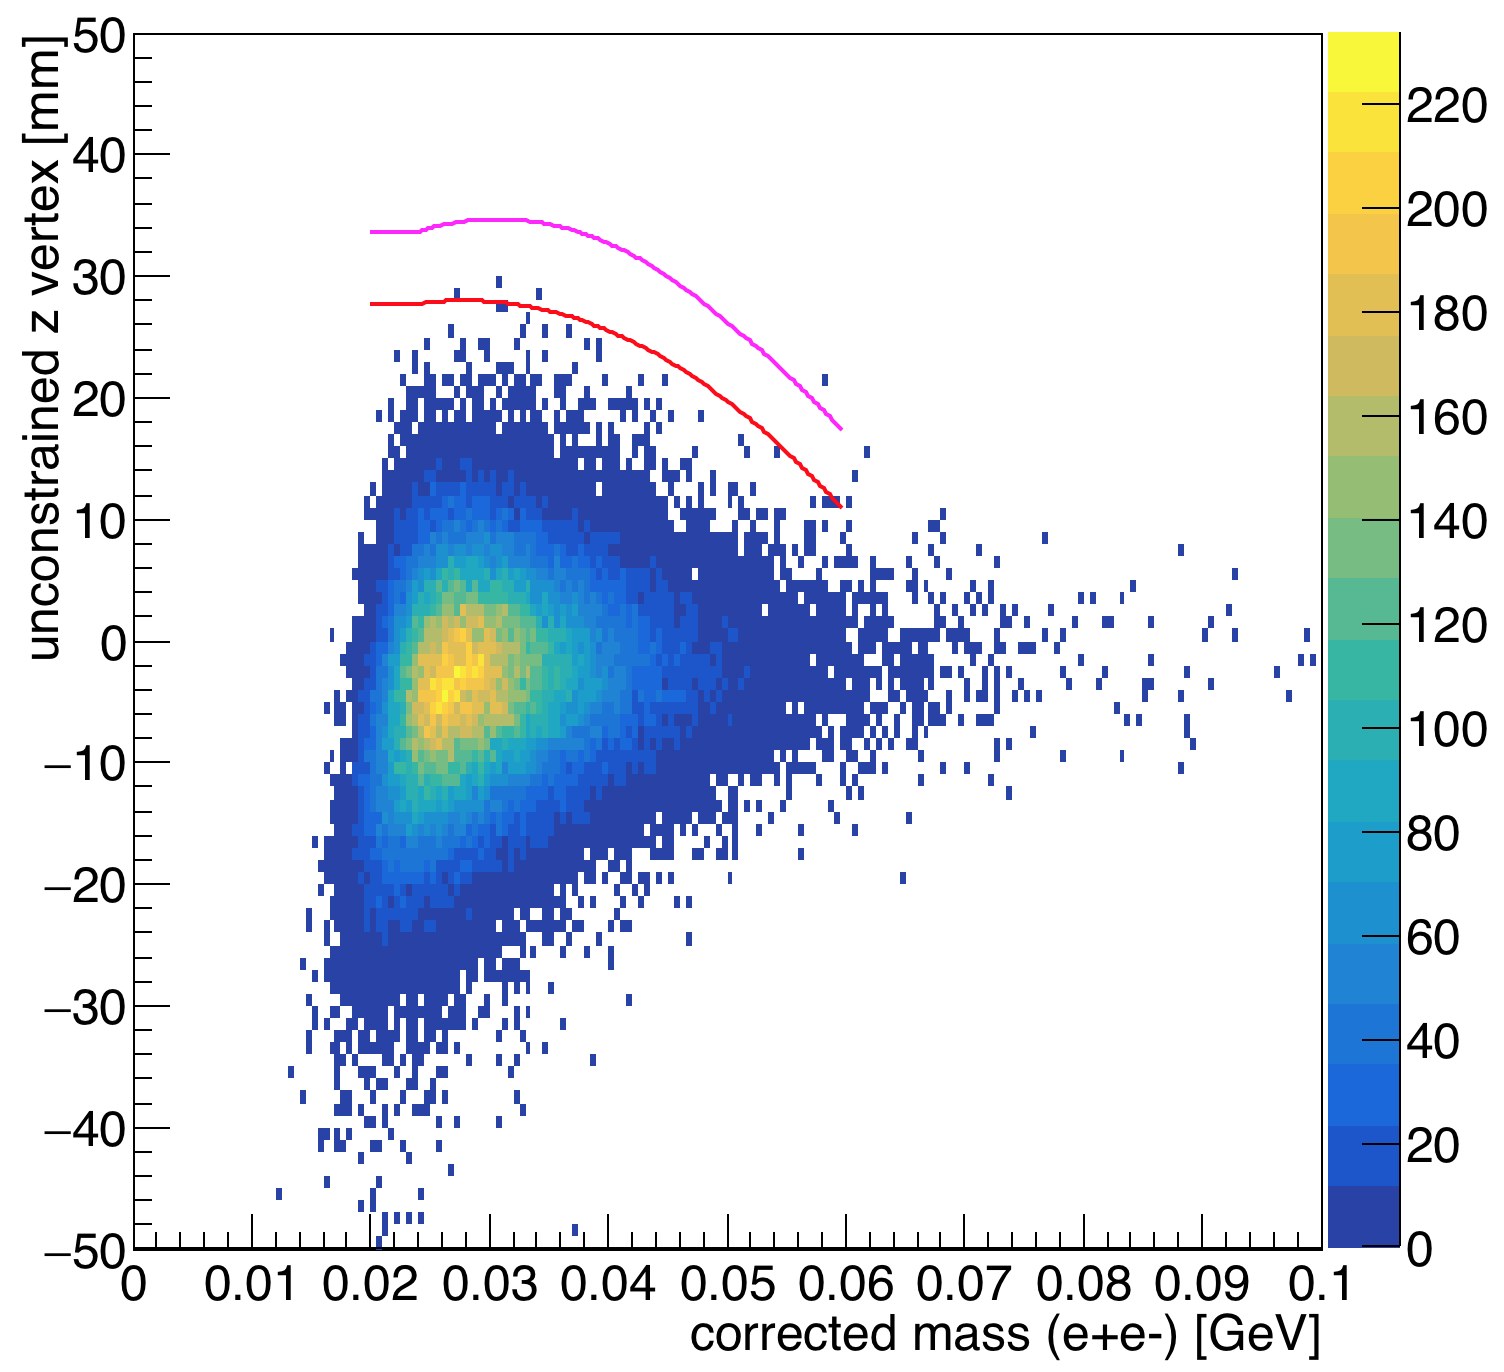
\includegraphics[width=\textwidth]{pics/appendix/zVm_L1L2_1p5_bl.png}
\end{minipage}\hfill\begin{minipage}{0.5\textwidth}
 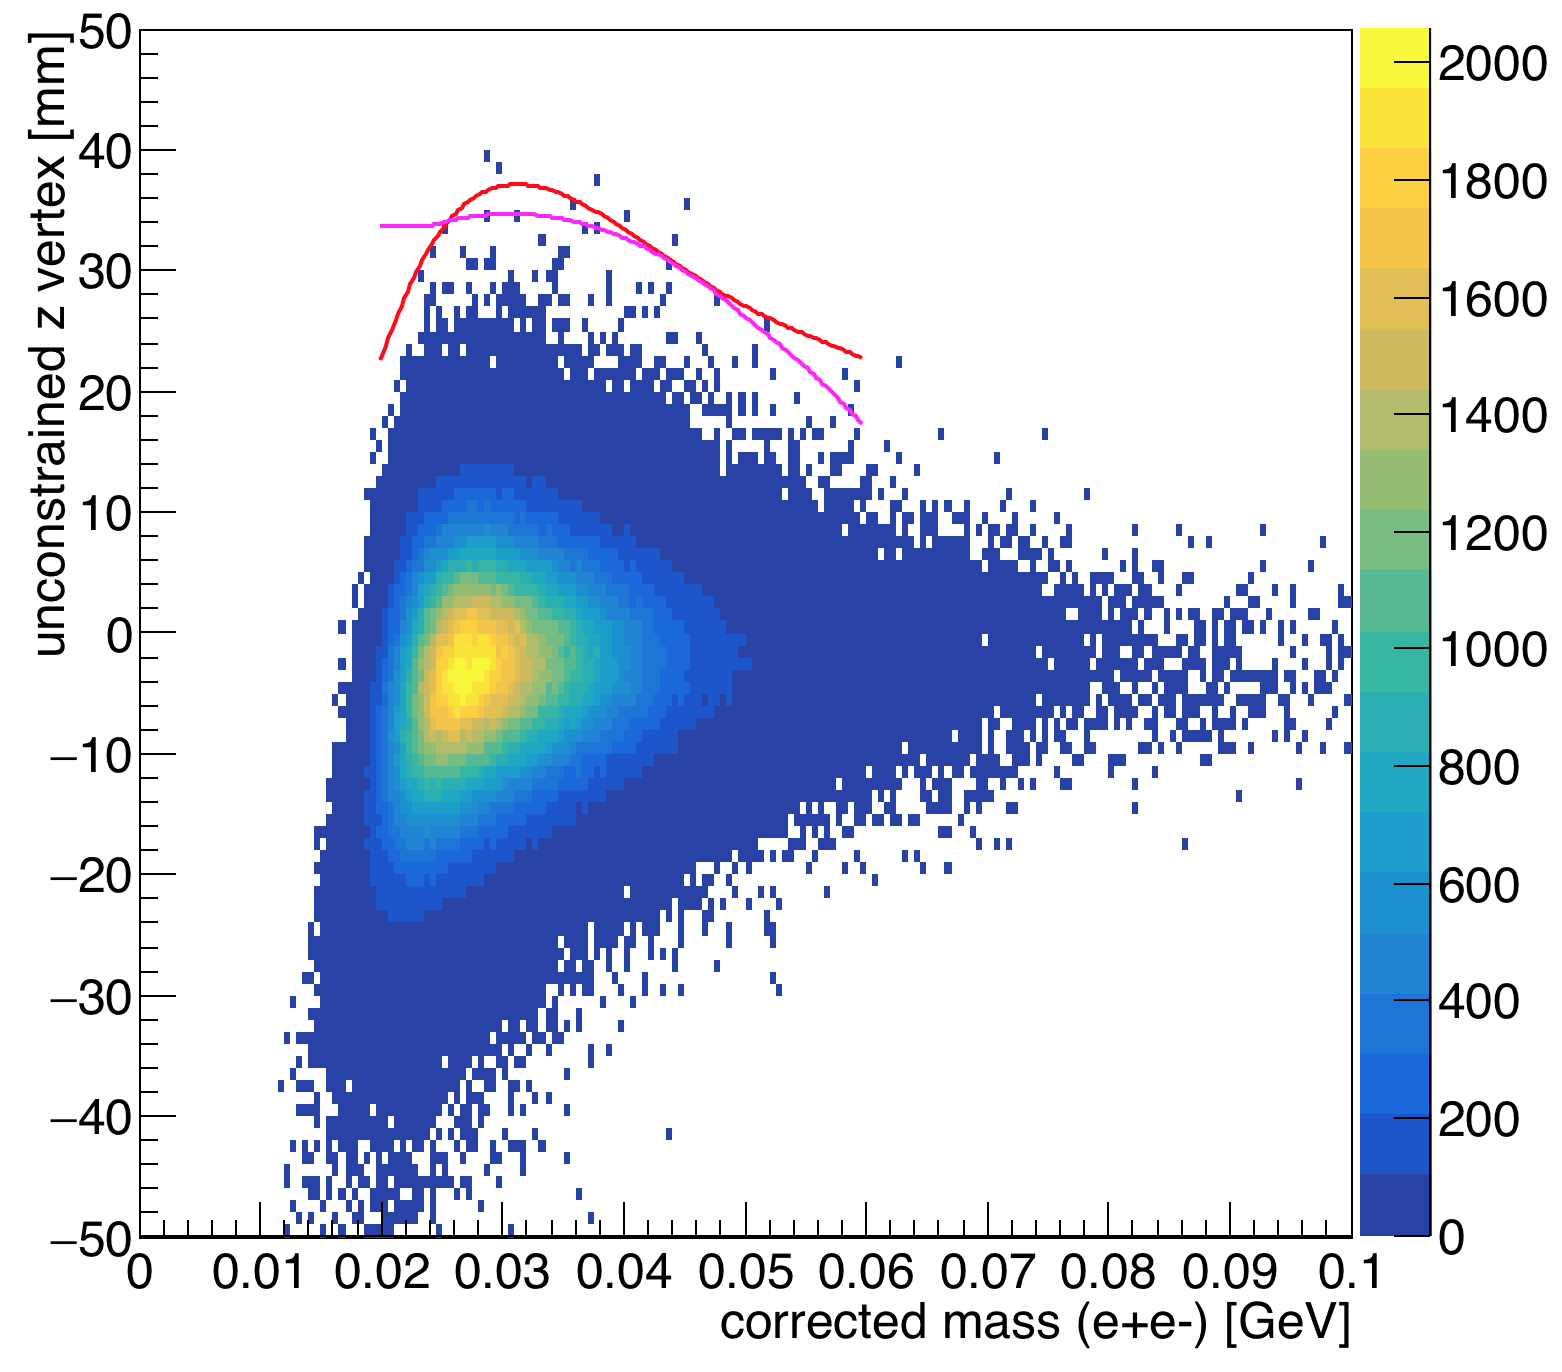
\includegraphics[width=\textwidth]{pics/appendix/zVm_L1L2_1p5_ub.png}
 \end{minipage}
  \caption[$z$ vertex and mass distribution for the L1L2 data set with the SVT at $\pm1.5$~mm]{The unconstrained $z$ vertex position for the L1L2 data set with the SVT at $\pm1.5$~mm is shown as a function of the corrected mass of the $e^+e^-$ pair where one track has a hit in Layer 1 and the other track does not pass through the active region of Layer 1. The $zCut$ as measured for this data is shown in red and corresponds to the full 100$\%$ data set where there is less than 0.5 background event beyond. The projected $zCut$ from the 10$\%$ of the data is shown in magenta. The relevant mass range used to measure $zCut$ is from 0.02--0.06~GeV based on measured statistics. The 10$\%$ sample for tuning cuts is shown on the left, and the full 100$\%$ of the data is shown on the right.}
  \label{fig:zvm_l1l2_1p5}
\end{figure}
\begin{figure}[htb]
  \centering
      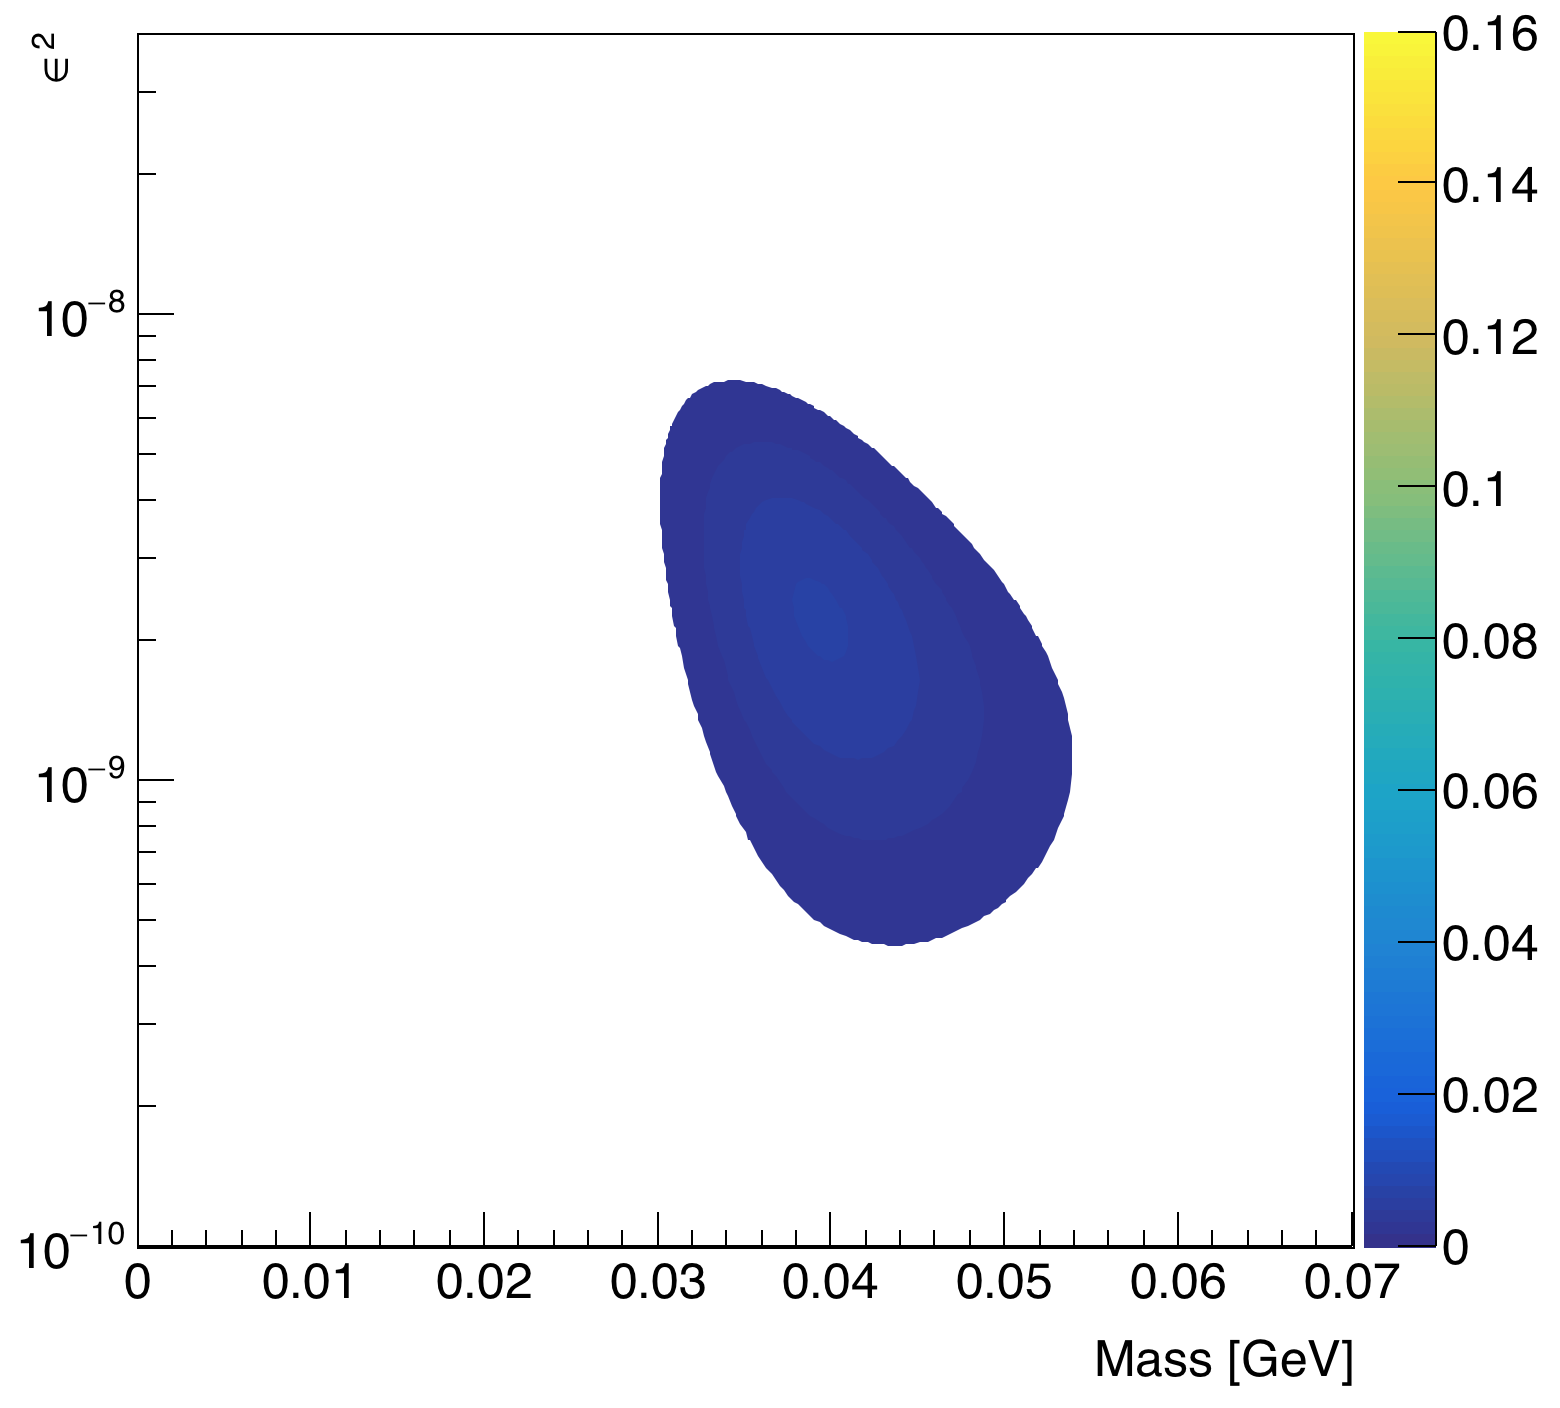
\includegraphics[width=0.5\textwidth]{pics/appendix/reachL1L2_1p5.png}
  \caption[Expected detectable $A^{\prime}$ signal yield from the L1L2 data at 1.5~mm.]{The expected number of detectable $A^{\prime}$ signal events for the L1L2 data set with the SVT at $\pm1.5$~mm is 0.007 events, and the distribution for coupling and mass space is shown. This calculation uses the $zCut$ from Figure~\ref{fig:zvm_l1l2_1p5}.}
  \label{fig:rl1l21p5}
\end{figure} 
\begin{figure}[hbt]
\begin{minipage}{0.5\textwidth}
 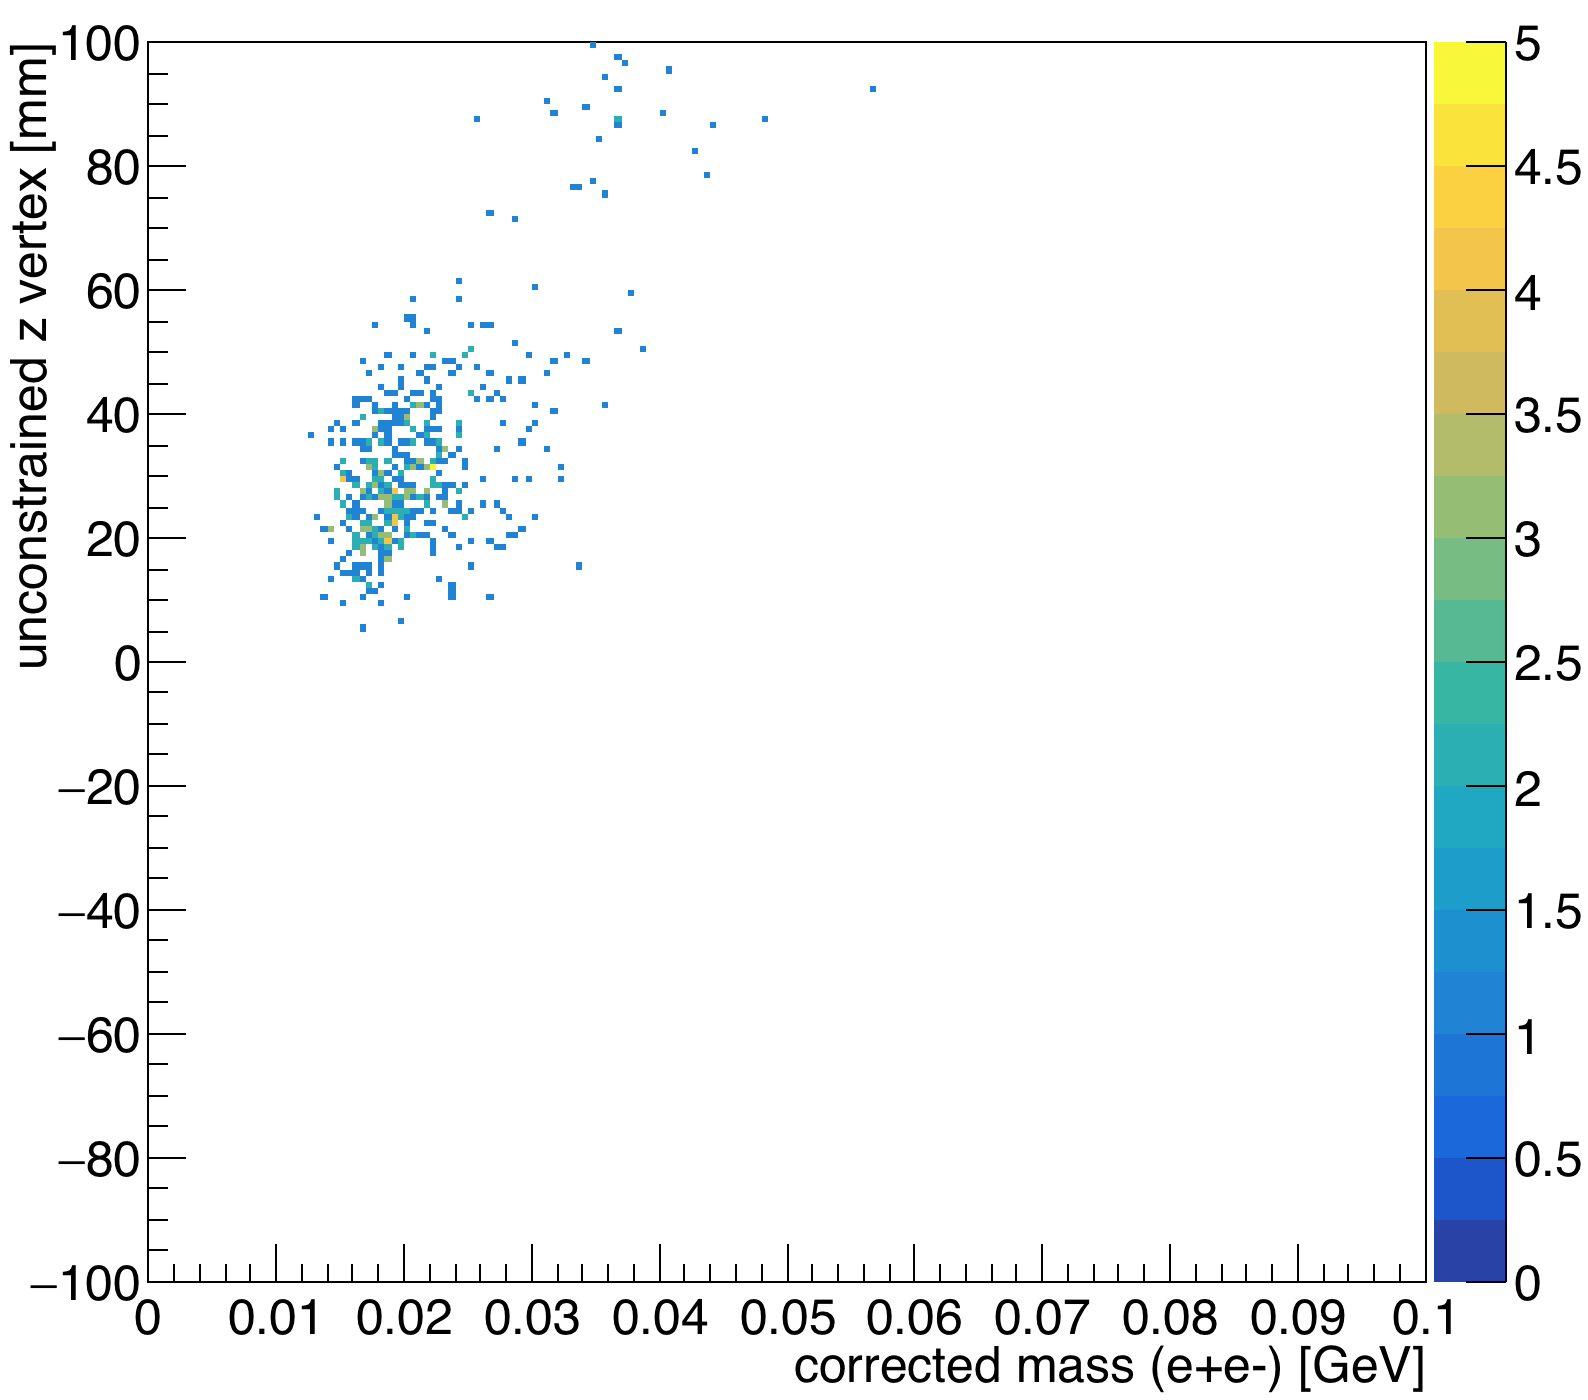
\includegraphics[width=\textwidth]{pics/appendix/zVm_L2L2_0p5_bl.png}
\end{minipage}\hfill\begin{minipage}{0.5\textwidth}
 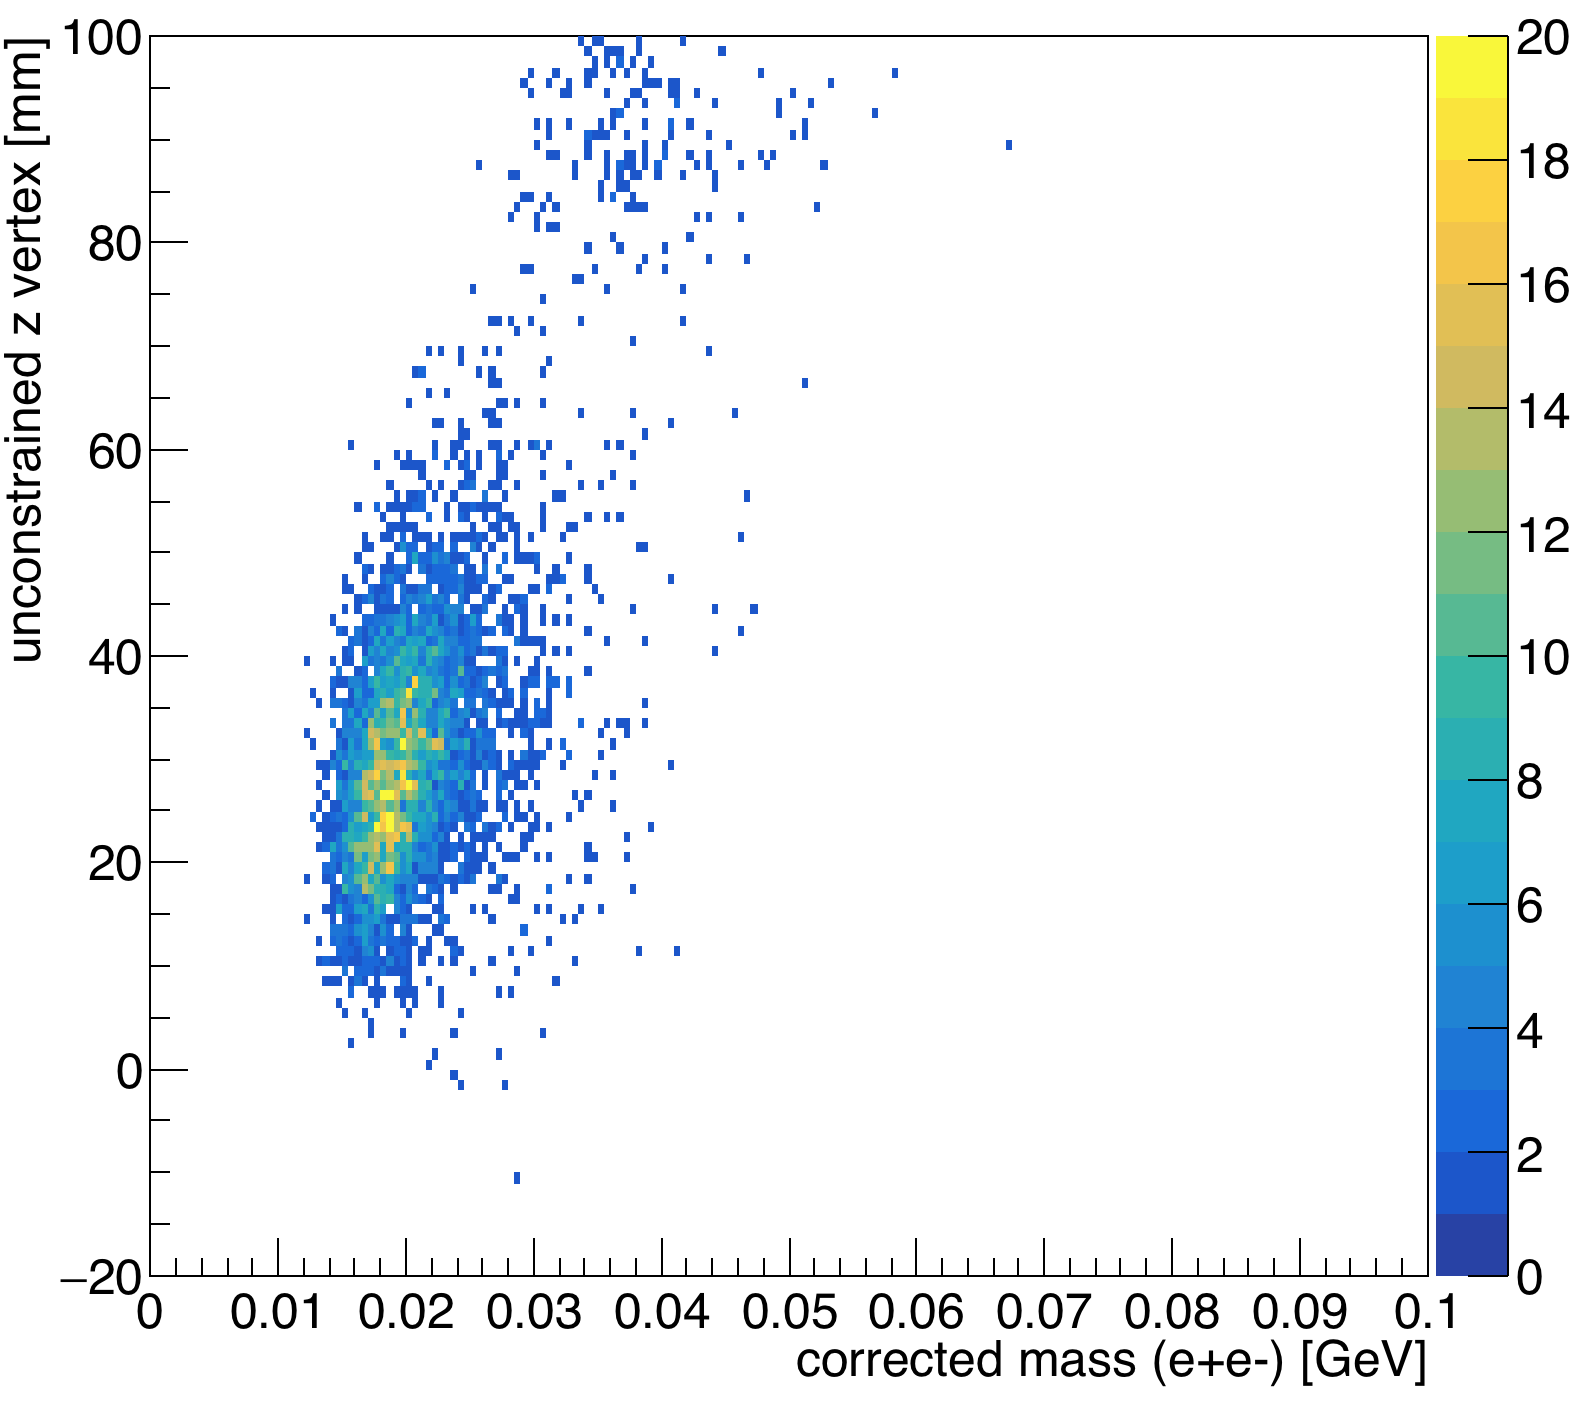
\includegraphics[width=\textwidth]{pics/appendix/zVm_L2L2.png}
 \end{minipage}
  \caption[$z$ vertex and mass distribution for the L2L2 data set with the SVT at $\pm0.5$~mm]{The unconstrained $z$ vertex position for the L2L2 data set with the SVT at $\pm0.5$~mm is shown as a function of the corrected mass of the $e^+e^-$ pair where both tracks do not pass through the active region of Layer 1. No $zCut$ is shown due to the presence of a large background extending to the downstream position of Layer 1.}
  \label{fig:zvm_l2l2}
\end{figure}
\begin{figure}[htb]
  \centering
      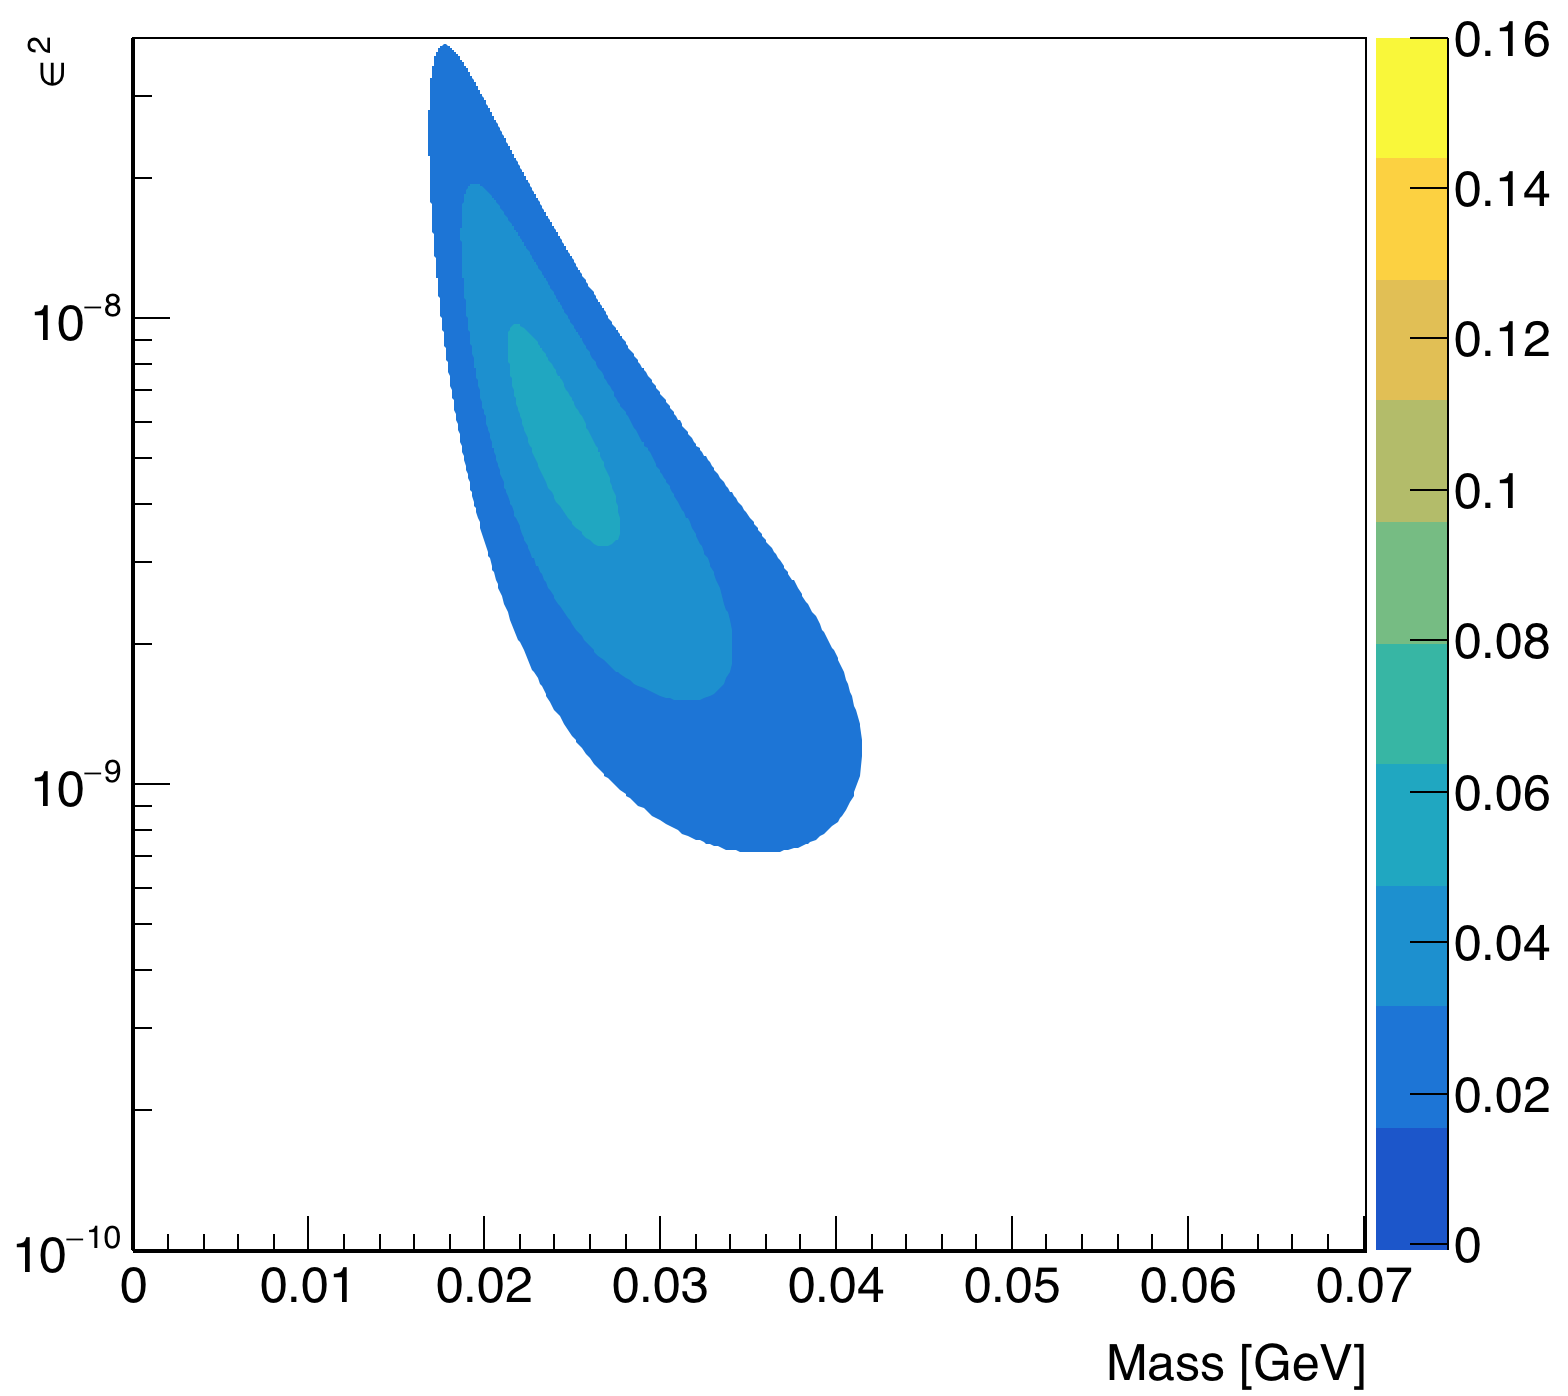
\includegraphics[width=0.5\textwidth]{pics/appendix/reachL2L2_0p5.png}
  \caption[Upper limit of the detectable $A^{\prime}$ signal from the L2L2 data at 0.5~mm]{The upper limit of detectable $A^{\prime}$ signal events from the L2L2 data set with the SVT at $\pm$0.5~mm is 0.05 events, assuming that all backgrounds can be removed and the $zCut$ can be optimally chosen to include all reconstructed vertex efficiency for the L2L2 data set. The distribution for coupling and mass space is shown.}
  \label{fig:rl2l20p5}
\end{figure} 
\begin{figure}[hbt]
\begin{minipage}{0.5\textwidth}
 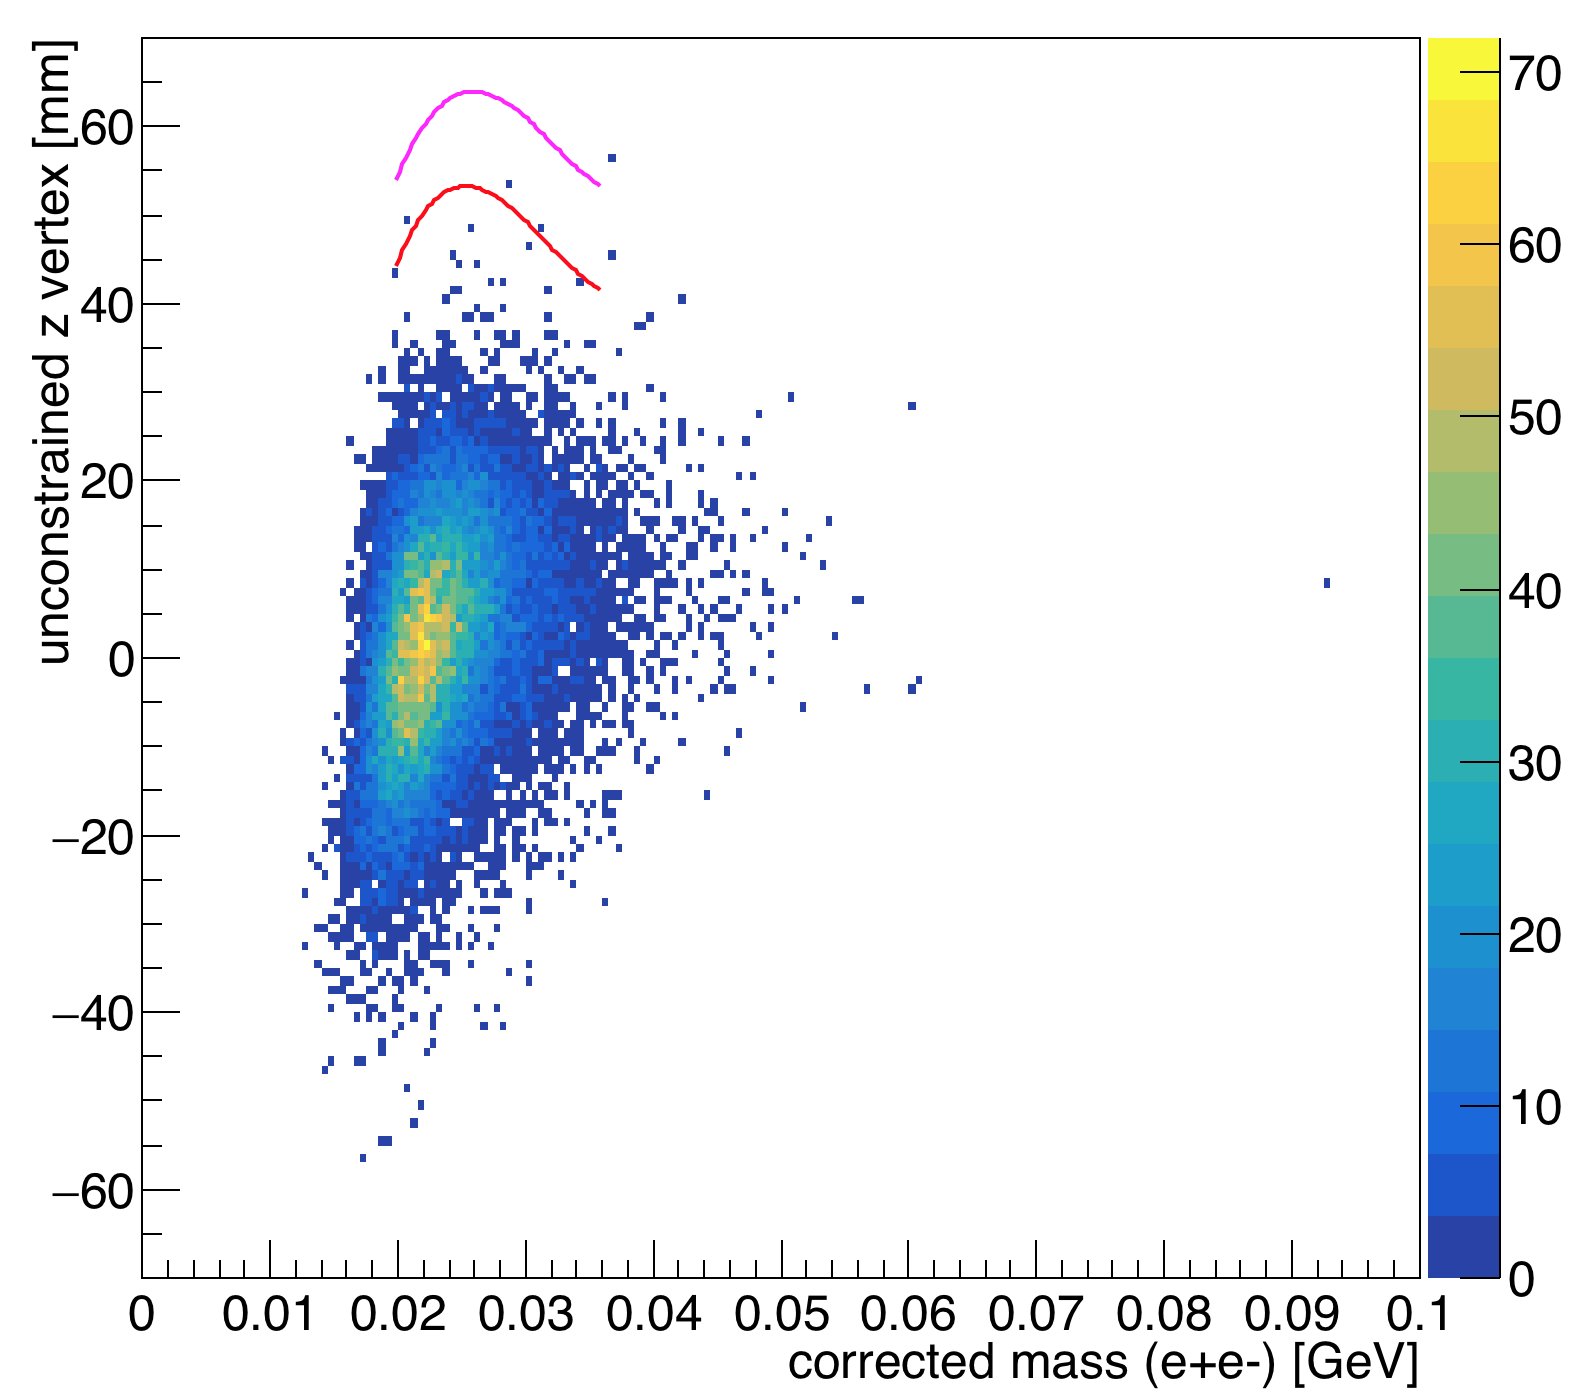
\includegraphics[width=\textwidth]{pics/appendix/zVm_L2L2_1p5_bl.png}
\end{minipage}\hfill\begin{minipage}{0.5\textwidth}
 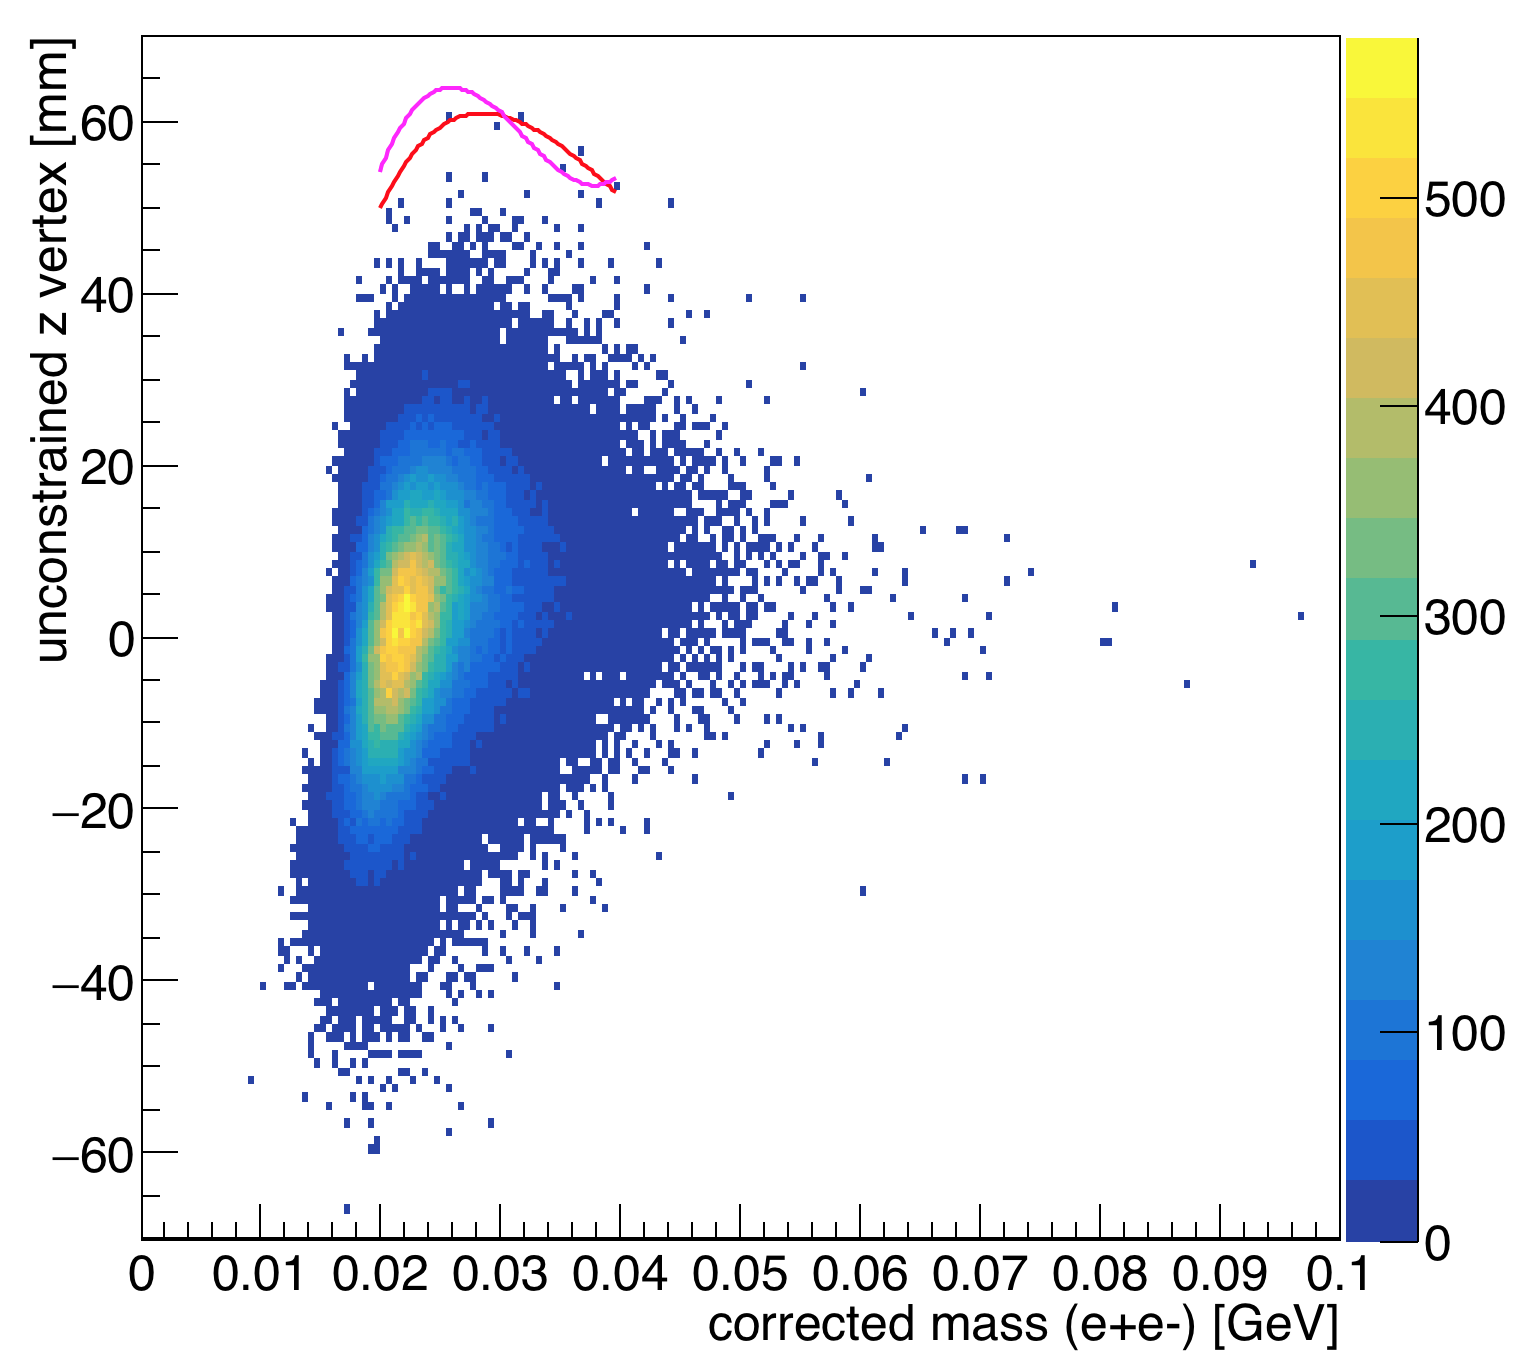
\includegraphics[width=\textwidth]{pics/appendix/zVm_L2L2_1p5_ub.png}
 \end{minipage}
  \caption[$z$ vertex and mass distribution for the L2L2 data set with the SVT at $\pm1.5$~mm]{The unconstrained $z$ vertex position for the L2L2 data with the SVT at $\pm1.5$~mm is shown as a function of the corrected mass of the $e^+e^-$ pair where both tracks do not pass through the active region of Layer 1. The $zCut$ as measured for this data is shown in red and corresponds to the full 100$\%$ data set where there is less than 0.5 background event beyond. The projected $zCut$ from the 10$\%$ of the data is shown in magenta. The relevant mass range used to measure $zCut$ is from 0.02--0.04~GeV based on measured statistics. The 10$\%$ sample for tuning cuts is shown on the left, and the full 100$\%$ of the data is shown on the right.}
  \label{fig:zvm_l2l2_1p5}
\end{figure}
\begin{figure}[htb]
  \centering
      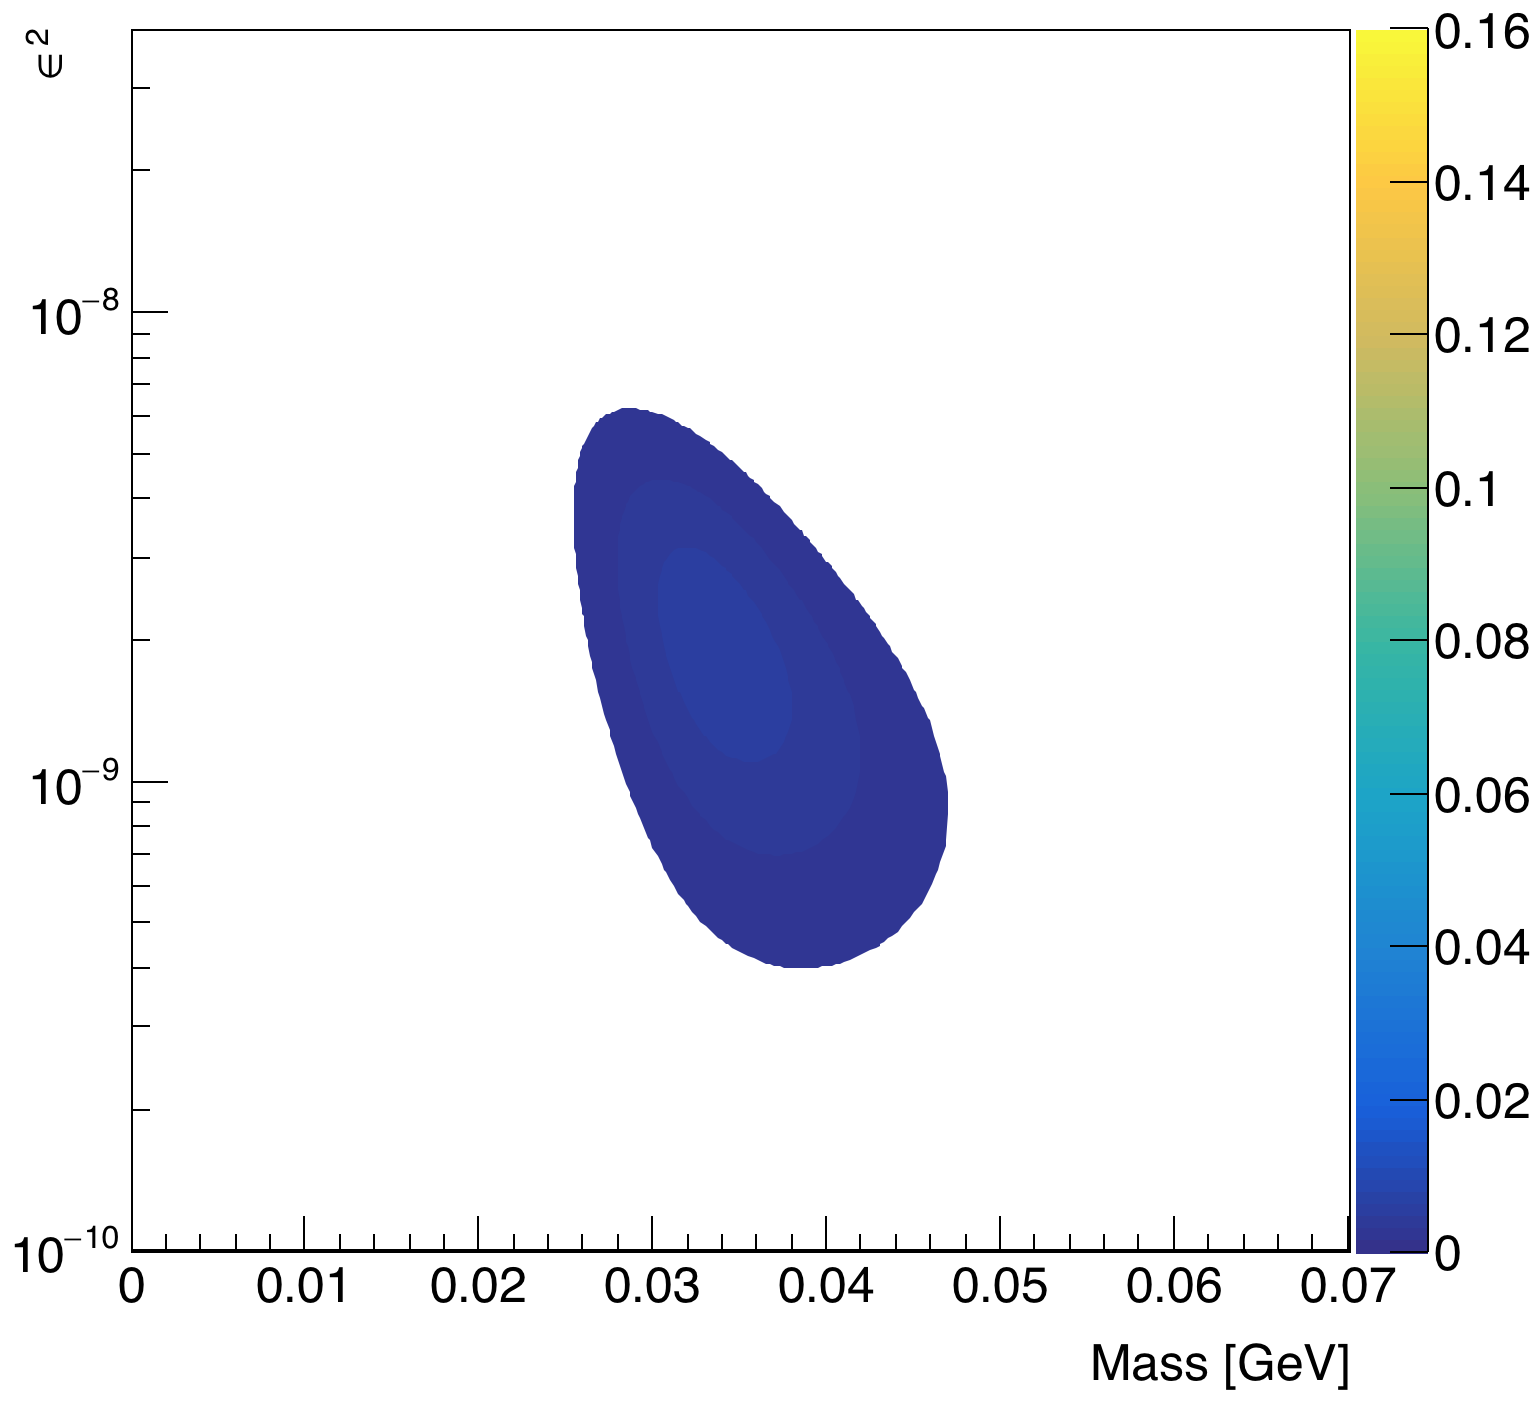
\includegraphics[width=0.5\textwidth]{pics/appendix/reachL2L2_1p5.png}
  \caption[Expected detectable $A^{\prime}$ signal yield from the L2L2 data at 1.5~mm]{The expected number of detectable $A^{\prime}$ signal events from the L2L2 data set with the SVT at $\pm1.5$~mm is 0.006 events, and the distribution for coupling and mass space is shown.}
  \label{fig:rl2l21p5}
\end{figure} 
The L1L2 data set requires one track to have passed through the active region of Layer 1 with a corresponding hit and the other track to have a first hit in Layer 2. To ensure that a track did not miss Layer 1 due to an inefficiency, the Layer 2 track is extrapolated to Layer 1 and verified that it did not pass through the active region of the silicon sensor. The mass and $z$ vertex distribution for the L1L2 data taken with the SVT at 0.5~mm is shown in Figure~\ref{fig:zvm_l1l2}. The L1L2 data forces the $zCut$ to be very high due to the presence of a large high $z$ background component. WAB conversions in Layer 1 generally have an electron in Layer 1 and the positron track in Layer 2 (missing Layer 1). This accounts for most of the statistics of this data. However, even if the data is divided for events where the electron has a hit in Layer 1 separately from when the positron has a hit in Layer 1, there are still large high $z$ backgrounds for each set that push the $zCut$ downstream. No one vertex cut (such as on the beam spot constraint quality or energy deposited in Layer 1) is able to remove these events. A $zCut$ closer to the target could restore some of the reach from this set, but the reach obtained is still much less than L1L1 data set. The expected number of signal events from the L1L2 data set is a maximum of 0.04 events and is shown in Figure~\ref{fig:rl1l20p5}.\\
\indent The mass and $z$ vertex distribution for the L1L2 data taken with the SVT at $\pm$1.5~mm is shown in Figure~\ref{fig:zvm_l1l2_1p5}. The corresponding expected $A^{\prime}$ signal yield is shown in Figure~\ref{fig:rl1l21p5}. As shown in both Figures~\ref{fig:zvm_l1l2} and~\ref{fig:zvm_l1l2_1p5}, the $zCut$ projection from the 10$\%$ data sample to the full 100$\%$ data is less consistent than the projection made for the L1L1 data sets. This is most likely due to the low statistics of these data sets which makes the projection from the fits less accurate.\\ 
\indent The L2L2 data sets are composed of vertexed pairs of tracks that missed Layer 1 and extrapolate to a region outside of the active silicon sensor at the Layer 1 position. The mass and $z$ vertex distribution for the L2L2 data taken with the SVT at 0.5~mm is shown in Figure~\ref{fig:zvm_l2l2}. The L2L2 data with the SVT at $\pm0.5$~mm from the beam is dominated by high $z$ backgrounds. This background extends to the $z$ position of the first SVT layer. Due to this background, this data set cannot contribute to the projected reach. Ideally, there should be no events in this data set except for pure signal events. These events cannot be $A^{\prime}$ signal alone due to their uniform distribution over several masses. If this high $z$ background can be removed, a $zCut$ should be chosen to optimize the reconstructed vertex efficiency. If the background events could be entirely removed, then the anticipated $A^{\prime}$ detectable signal yield is shown in Figure~\ref{fig:rl2l20p5}. The maximum number of detectable signal events (as an upper limit) that this data set could contribute to the reach is 0.05 events, assuming all backgrounds could be removed.\\
\indent The L2L2 data with the SVT slightly more open at $\pm1.5$~mm from the beam is shown in Figure~\ref{fig:zvm_l2l2_1p5}. The $zCut$ from the L2L2 data at 1.5~mm is pushed relatively far downstream due to the large number of events that decayed after the target. Due to the far downstream $zCut$ and low statistics of the 1.5~mm data, the expected $A^{\prime}$ signal yield shown in Figure~\ref{fig:rl2l20p5} does not contribute significantly to the overall reach for all combined data sets. 
